\chapter{Requisitos y casos de uso}
\section{Requisitos candidatos}
\par En primer lugar se identifican los requisitos que se intentarán cumplir con la solución propuesta.
\par Se agrupan los requisitos según estén más orientados al componente WAF o al componente de TLS.
\par Requisitos orientados principalmente al componente WAF:
\begin{enumerate}[\bfseries{WAF-}Req1. ]
  \item \label{req:independence} La solución debe poder ejecutarse en un sistema operativo o máquina independiente de la plataforma de la aplicación web con el
    objetivo de garantizar independencia en las tareas de administración y permitir aplicar un modelo RBAC.

  \item \label{req:commonattacks} La solución debe disponer de un conjunto básico de políticas de auditoría o bloqueo que permitan proteger la aplicación web
    frente a los ataques más comunes.

  \item La plataforma debe permitir implementar parches virtuales frente a ataques conocidos.

  \item La solución debe permitir la elaboración de reglas personalizadas según las necesidades específicas de la plataforma del cliente.

  \item \label{req:softwarelibre} La plataforma debe ser compatible con el modelo de licencias de {\em software libre\cite{softwarelibre}} tipo Licencia Pública
    General de GNU (en adelánte \acrshort{gpl}, de  sus siglas en inglés \acrlong{gpl}, licencia \cite{gpl}) o Licencia Pública General Reducida de GNU (en adelánte \acrshort{lgpl},
    de sus siglas en inglés \acrlong{lgpl}, licencia \cite{lgpl}).

  \item \label{req:facilidad} La plataforma debe ser fácilmente integrable en la plataforma web del cliente.
    \par Tal como se ha detallado en la sección ~\nameref{subsec:estadoarte}, el despliegue y la operación de los WAF de software libre es complejo, y esta complejidad es uno de las causas de su escasa adopción. Es por ello que se considera de
    vital importancia para su adopción que la solución ofrecida sea fácil de desplegar u operar. Para ello, un factor determinante es minimizar los cambios necesarios en la infraestructura previa y  las actividades de administración de la
    plataforma.

  \item \label{req:escalado} Escalabilidad. La plataforma debe permitir la ampliación o reducción de recursos de forma dinámica. Debido a que la solución está situada entre la plataforma web y las peticiones de los clientes, es clave que la
    solución WAF pueda ampliarse o reducirse según sea necesario.

  \item La plataforma debe generar logs de seguridad exportables a soluciones externas de gestión de información y eventos de seguridad (en
    adelante \acrshort{siem} de sus siglas en inglés, \acrlong{siem}).
\end{enumerate}

\par A continuación se recogen los requisitos asociados al componente de TLS:
\begin{enumerate}[\bfseries{TLS-}Req1. ]
  \item \label{req:tls} La solución debe poder participar en la negociación TLS, presentando certificados confiables a los clientes.

  \item La solución deber poder gestionar los certificados presentados a los clientes incluyendo soporte a la extensión \acrshort{SNI} de TLS.

  \item La plataforma debe soportar TLS versión 1.3, HTTP/2 y otros elementos incluidos en las {\em buenas prácticas de TLS\cite{TLSBestPractices}}.

  \item Debe permitir aplicar soluciones de SSL offloading, entre el WAF y los frontales de la plataforma web, o permitir cifrado punto a punto.
    \par En caso de utilizar la funcionalidad de SSL offloading:
      \begin{enumerate}[label=\emph{\alph*})]
        \item Esta opción es recomendable en entornos controlados en los que prima el rendimiento.
        \item Las comunicación entre el WAF y la plataforma web debe permitir tráfico HTTP.
      \end{enumerate}
    \par En caso de cifrado punto a punto:
      \begin{enumerate}[label=\emph{\alph*})]
        \item Esta opción es recomendable en las soluciones en las que prime la seguridad o en aquellos escenarios en los que no se tenga el control de
          elementos intermedios, como por ejemplo en entornos Cloud o multi-datacenter.
        \item Las comunicación entre el WAF y la plataforma web debe permitir tráfico HTTPS.
        \item El WAF debe confiar en la CA que firma los certificados de la plataforma web o, alternativamente, en los certificados hoja.
      \end{enumerate}
\end{enumerate}

\section{Identificación de actores}
\par Se han identificado los siguientes actores (algunos de ellos se identifican también en inglés debido a que múltiples referencias los mencionan en inglés).
\begin{itemize}
  \item {\bf Cliente (Client en inglés)}. Se utiliza este término para referirse al cliente web que consume los servicios HTTP o HTTPS.
  \item {\bf \Gls{Atacante} (Black Hat Hacker en inglés)}. Se trata de un tipo de cliente malintencionado.
  \item {\bf Plataforma web (Web Servers en inglés)}. Se considera toda la infraestructura necesaria para servir los contenidos web. En esta infraestructura no
    se incluyen los elementos desarrollados en el presente proyecto.
  \item {\bf Autoridad de certificación} (en adelante \GLS{CA}). Es el elemento encargado de firmar los certificados TLS. El cliente debe confiar en la CA o en los certificados hoja alternativamente. En caso de cifrado punto a punto el WAF deberá confiar en los certificados presentados por la plataforma web.
  \item {\bf Plataforma WAF+TLS}. Se trata de la plataforma propuesta en el presente proyecto.
\end{itemize}

\clearpage
\section{Casos de uso}
\par Estos son los casos identificados.
\begin{enumerate}
  \item Caso de uso: Petición identificada como legítima de recurso web.
    \begin{itemize}
      \item Actores: Cliente, plataforma web, plataforma WAF+TLS.
      \item Descripción: Se trata del caso de uso que sucede con mayor frecuencia, pues representa las peticiones legítimas de clientes a la plataforma web. Se pueden representar las comunicaciones en los siguientes pasos:
        \begin{enumerate}
          \item El cliente realiza una petición web a la solución propuesta en el presente proyecto.
          \item La plataforma WAF+TLS evalúa la petición, la considera legítima y la envía a la plataforma web.
          \item La plataforma web recibe la petición y envía una respuesta a la plataforma WAF+TLS.
          \item La plataforma WAF+TLS recibe la respuesta y se la envía al cliente.
        \end{enumerate}
        \par Se debe tener en cuenta que en este caso de uso se incluyen peticiones legítimas y falsos negativos cuando el WAF falla al detectar un ataque.
      \item Diagrama:
        \begin{center}
          \label{fig:CasoUso1}
          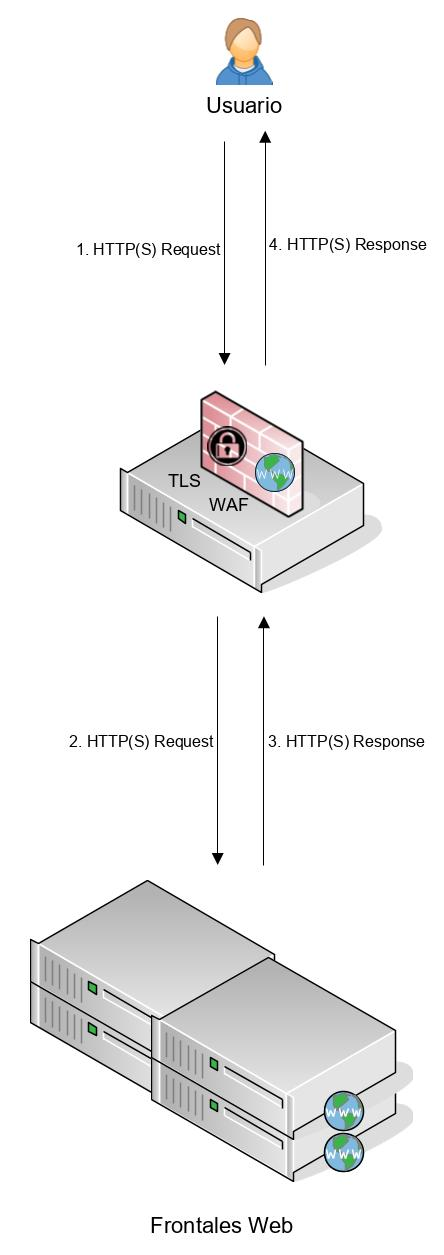
\includegraphics[width=0.3\textwidth]{fig/UseCase1}
        \end{center}
    \end{itemize}
\clearpage
  \item Caso de uso: Petición identificada como no legítima de recurso web.
    \begin{itemize}
      \item Actores: \Gls{Atacante}, plataforma WAF+TLS.
      \item Descripción: Este caso de uso se dará siempre que la plataforma WAF+TLS reciba una petición y la considere un ataque. En este caso se pueden identificar los siguientes pasos:
        \begin{enumerate}
          \item El atacante realiza una petición web a la plataforma WAF+TLS.
          \item La plataforma WAF+TLS recibe la petición, la evalúa y, considerándola como ataque, envía un mensaje de error al atacante.
        \end{enumerate}
        \par A tener en cuenta que la plataforma WAF+TLS ha considerado que el cliente es un atacante y este caso de uso se dará tanto en ataque reales como con falsos positivos (cuando se diagnostica como ataque a una
        petición legítima).
      \item Diagrama:
        \begin{center}
          \label{fig:CasoUso2}
          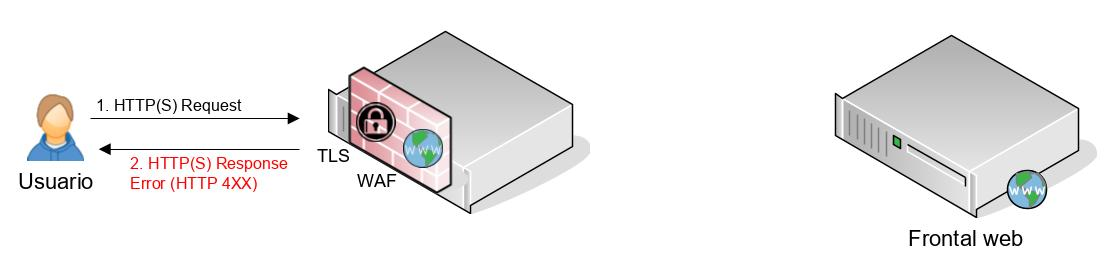
\includegraphics[width=0.3\textwidth]{fig/UseCase2}
        \end{center}
    \end{itemize}
\clearpage
  \item Caso de uso: Petición HTTPS en un entorno con TLS offloading.
    \begin{itemize}
      \item Actores: Cliente, plataforma web, plataforma WAF+TLS.
      \item Descripción: Se trata de una derivada del Caso de primer caso de uso. En este escenario las peticiones HTTPS realizadas por el cliente se envían sin cifrar (o en texto plano) a la plataforma web.
        \par Con ello se consigue reducir la carga que debe soportar la plataforma web y optimizar sus recursos.
        \par Sin embargo, también se aumenta el riesgo a un ataque en caso de que un potencial atacante tuviese acceso a la infraestructura situada entre la solución WAF y la plataforma web. Es por ello que esta solución
        sólo se recomienda en escenarios en los que los elementos situados entre ambos estén protegidos y monitorizados adecuadamente.
      \item Diagrama:
        \begin{center}
          \label{fig:CasoUso3}
          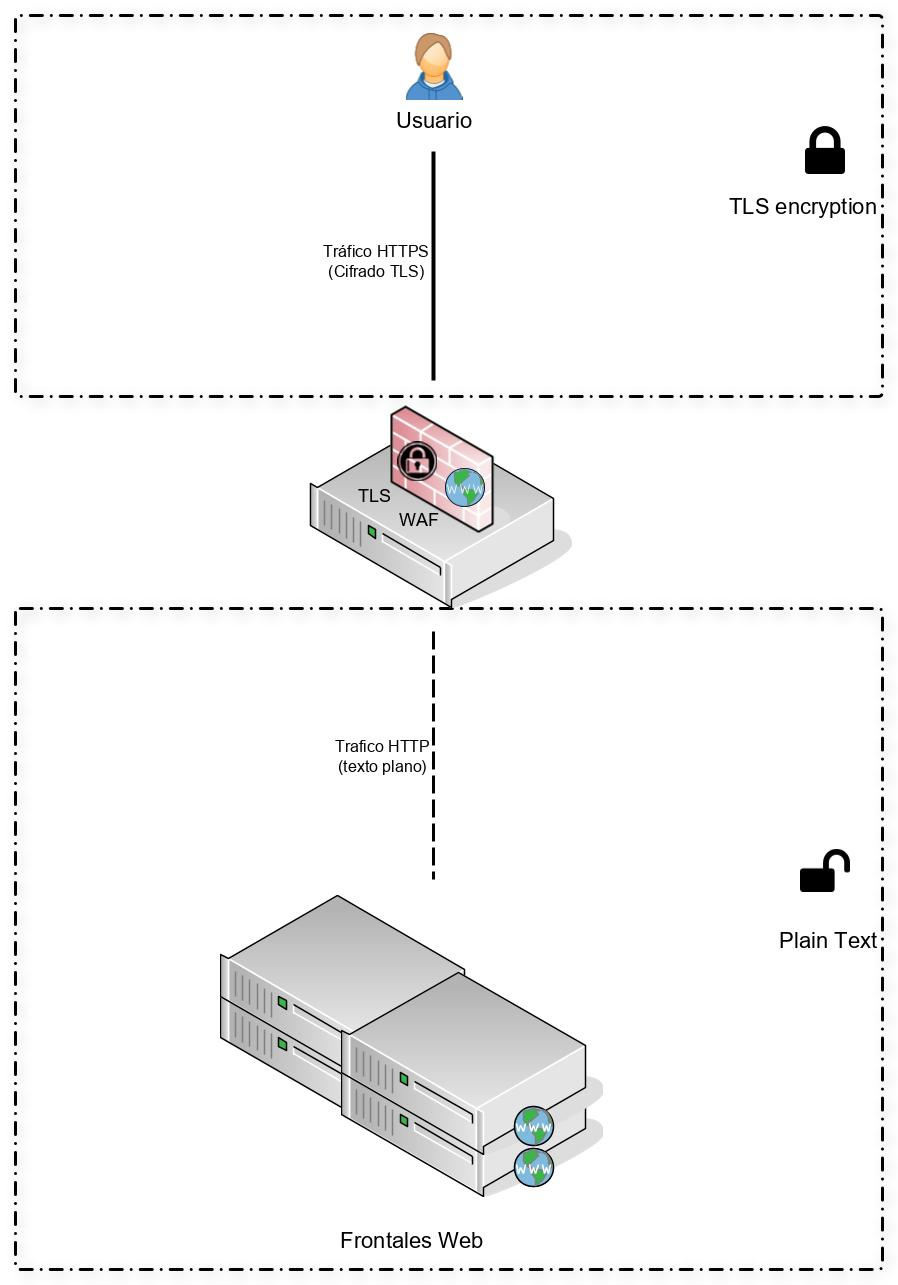
\includegraphics[width=0.7\textwidth]{fig/UseCase3}
        \end{center}
    \end{itemize}
\clearpage
  \item Caso de uso: Petición HTTPS con cifrado punto a punto.
    \begin{itemize}
      \item Actores: Cliente, plataforma web, plataforma WAF+TLS.
      \item Descripción: Se trata de un caso de uso alternativo al anterior. En este escenario se mantienen las comunicaciones cifradas también entre el WAF y la plataforma web, con lo que se consigue el cifrado punto a punto.
        \par Para ello se establecen dos túneles TLS: El primero entre el cliente y la plataforma WAF y un segundo túnel entre el WAF y la plataforma web.
      \item Diagrama:
        \begin{center}
          \label{fig:CasoUso4}
          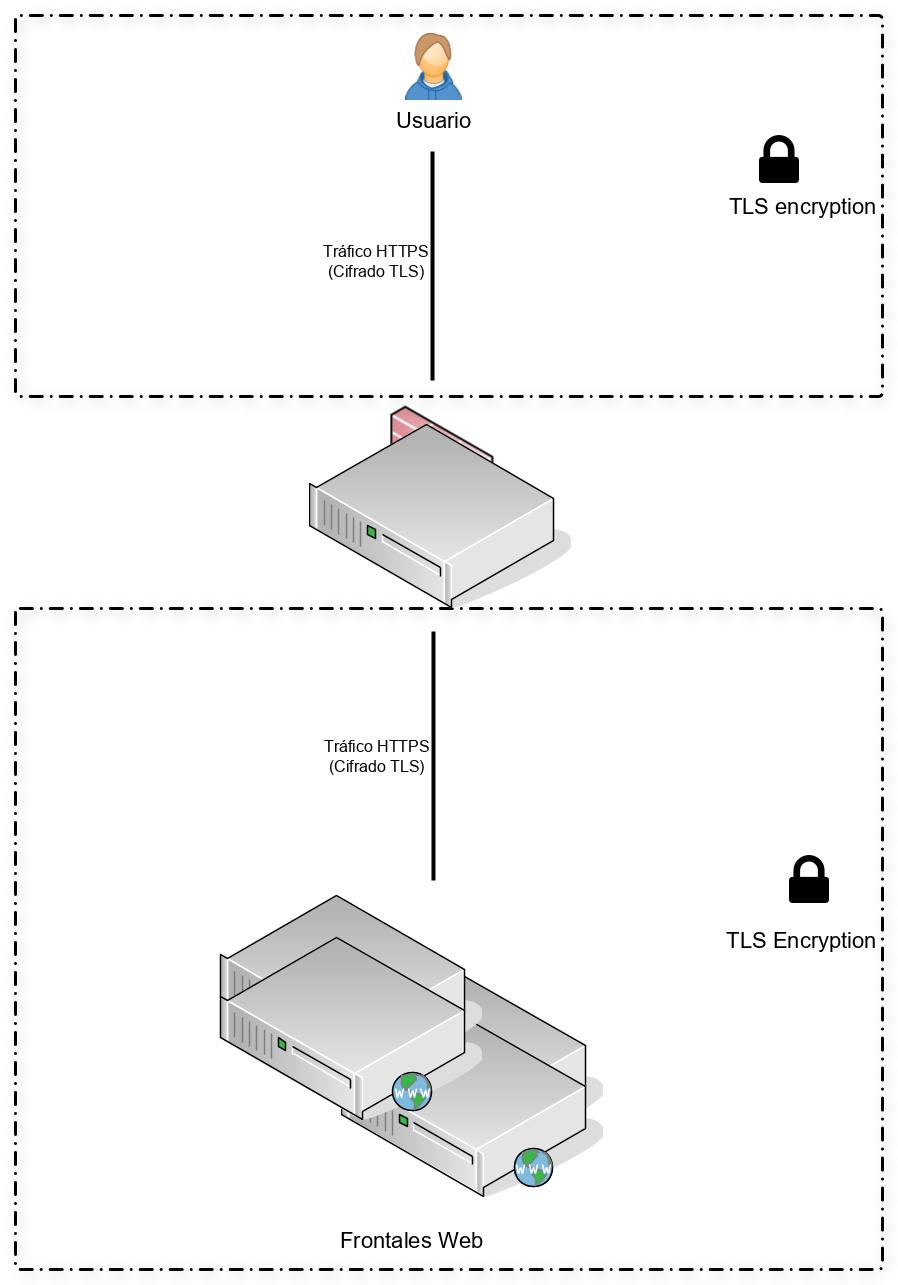
\includegraphics[width=0.7\textwidth]{fig/UseCase4}
        \end{center}
    \end{itemize}
\clearpage
  \item Caso de uso: Petición de validación y firma de certificado TLS a una CA de confianza.
    \begin{itemize}
      \item Actores: \acrlong{ca}, plataforma WAF+TLS.
      \item Descripción: Este caso de uso tiene como objetivo obtener un certificado digitalmente por una \acrshort{ca} que sea de confianza para el cliente. Se puede dividir en dos flujos similares.
        \par El primer flujo se da entre el WAF y la CA siguiendo los siguientes pasos:
        \begin{enumerate}
          \item El WAF - o un administrador del WAF - genera un certificado CSR~\cite[Wikipedia]{wiki:csr} asociado a su clave privada que siga el {\em estándar X.509 v3~\cite[IETF 5280]{rfc5280}}.
          \item Se envía el certificado a la CA solicitando que ésta lo firme.
          \item La CA valida que la petición es legítima y firma el certificado con su clave raíz o, alternativamente, una clave intermedia.
          \item La CA envía el certificado firmado digitalmente el WAF.
          \item Una vez el WAF disponga de dicho certificado, este puede presentar sus servicios web a los clientes y estos podrán validar al WAF durante la negociación TLS si confían en el certificado raíz de la CA o en la
            jerarquía de certificados.
        \end{enumerate}
        \par El segundo flujo es opcional. Se trataría de un flujo similar al descrito para el WAF pero el solicitante de certificado sería la plataforma web en este caso.
        \par Se considera que es opcional debido a que la plataforma web sólo estará expuesta al WAF y se podría crear una relación de confianza sin necesidad de hacer uso de una CA externa.
        \par No obstante, dado que actualmente obtener este tipo de certificados no tiene un coste económico, y que tampoco debería tener un impacto operacional significativo, se recomienda seguir el mismo proceso que para el WAF y
        hacer uso de certificados firmados digitalmente por un CA.
        \par En este proyecto, para la gestión de certificados del WAF se intentará hacer uso del protocolo \acrshort{acme} (\acrlong{acme}) mediante {\em Let’s Encrypt~\cite{letsencrypt}} con el objetivo de automatizar las
        actividades de creación y renovado de certificados.
      \item Diagrama:
        \begin{center}
          \label{fig:CasoUso5}
          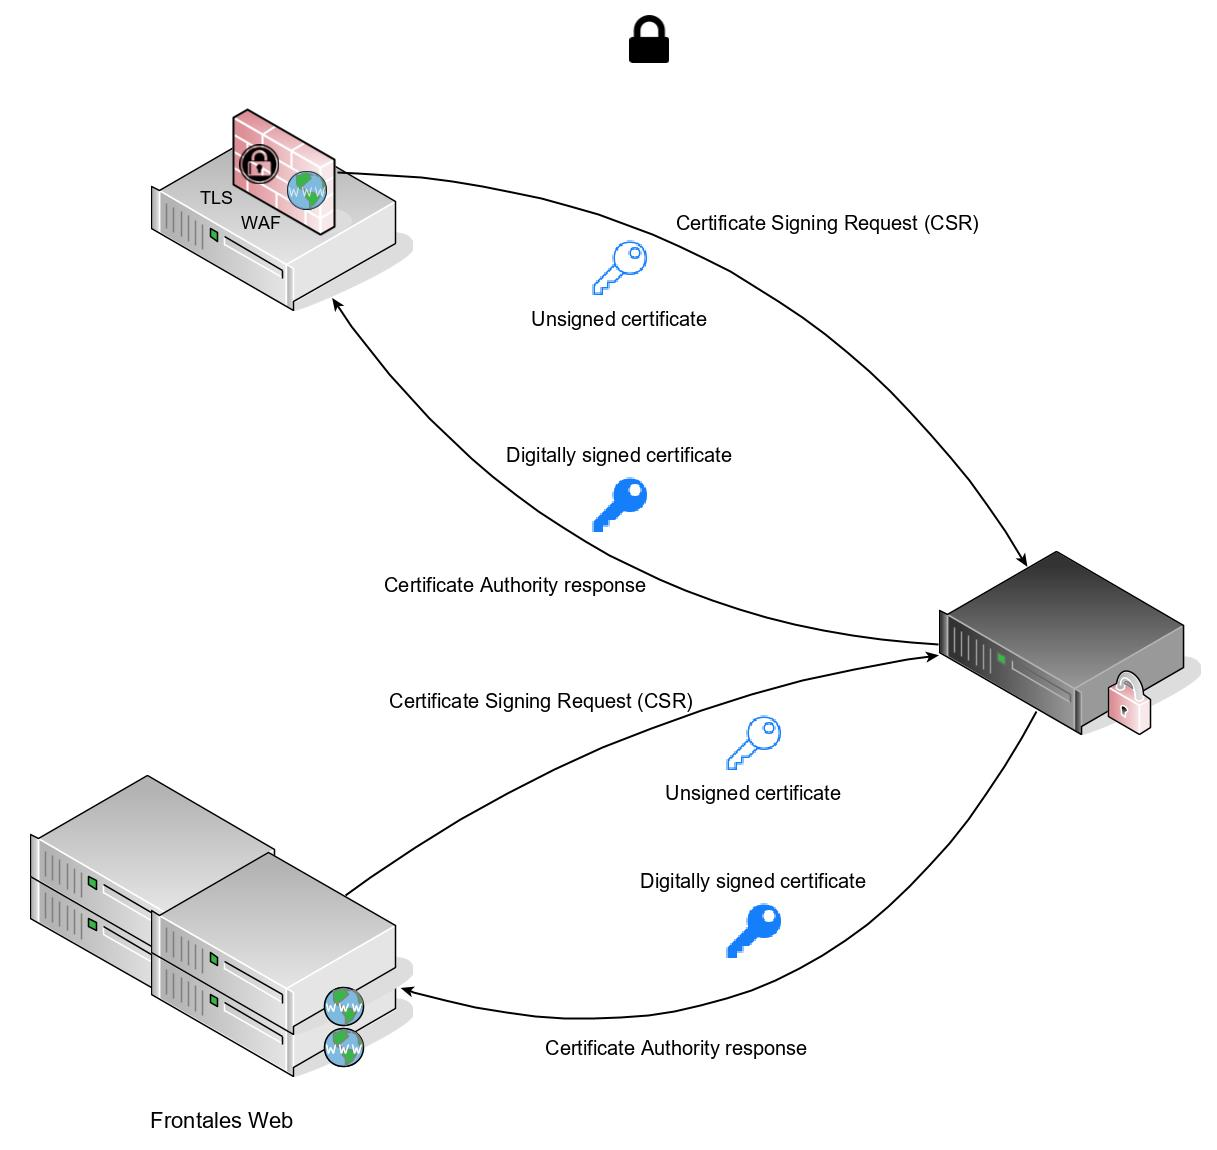
\includegraphics[width=0.7\textwidth]{fig/UseCase5}
        \end{center}
    \end{itemize}
\end{enumerate}


